\section{Voxelización} % (fold)
\label{sec:voxelizacion}
El trazado de conos contra geometría poligonal compleja es costoso. Encontrar los puntos de intersección entre un cono y un polígono es mucho más complejo que intersecciones rayo-polígono, además de esto un solo cono podría intersectar muchos polígonos.

Para simplificar el trazado de conos se utiliza una discretización de la escena en forma de vóxeles. Esta representación puede ser filtrada a niveles más bajos de detalle. Esto nos permite aproximar el efecto de extensión sobre la apertura del cono utilizando cada vez un nivel de detalle más bajo a través del recorrido del mismo.

\begin{figure}[H]
	\centering
	\begin{subfigure}[b]{.32\linewidth}
		\centering
		\captionsetup{justification=centering}
		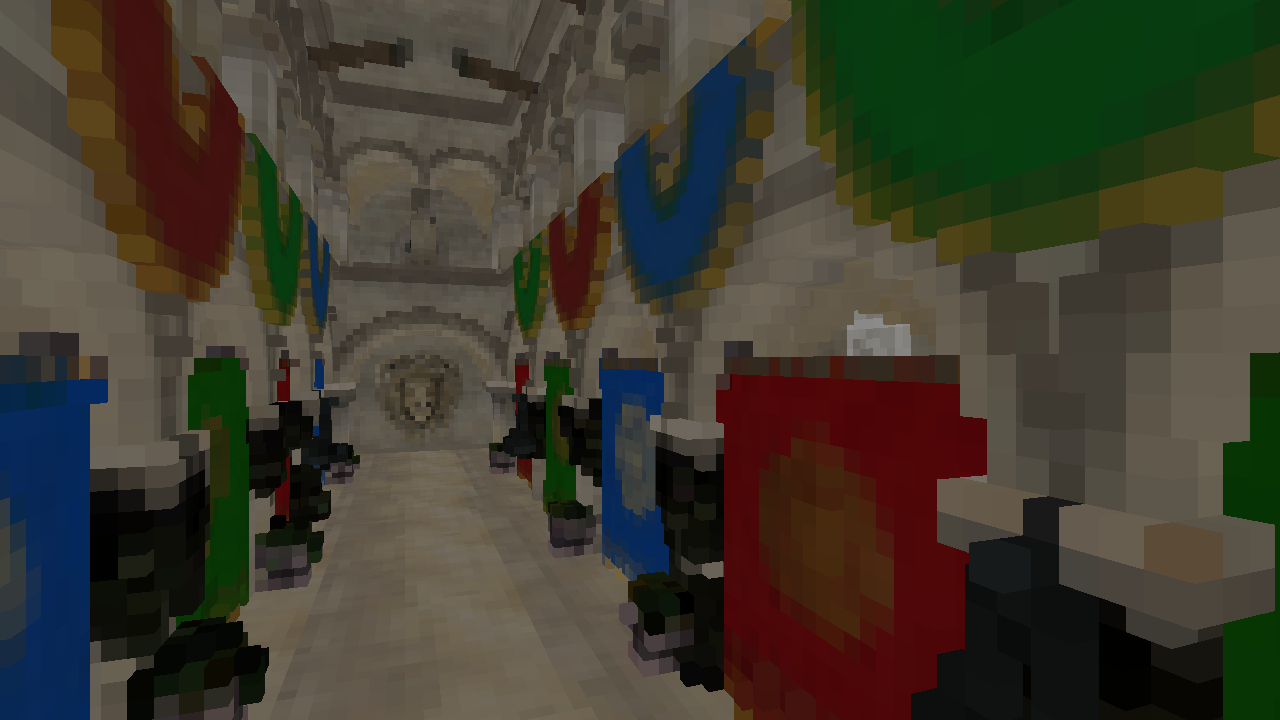
\includegraphics[width=\linewidth]{media/finals/albedo_v256.png}
	\end{subfigure}%
	\hspace{0.01\textwidth}
	\begin{subfigure}[b]{.32\linewidth}
		\centering
		\captionsetup{justification=centering}
		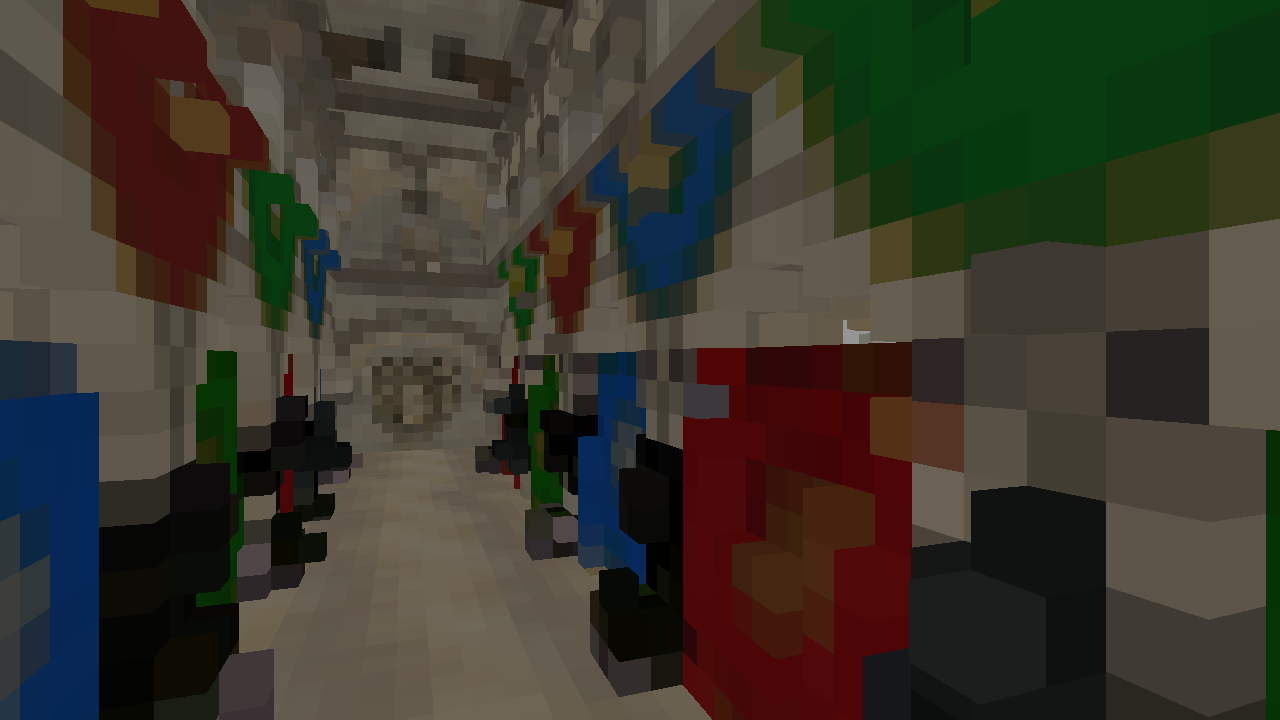
\includegraphics[width=\linewidth]{media/finals/albedo_v128.png}
	\end{subfigure}%
	\hspace{0.01\textwidth}
	\begin{subfigure}[b]{.32\linewidth}
		\centering
		\captionsetup{justification=centering}
		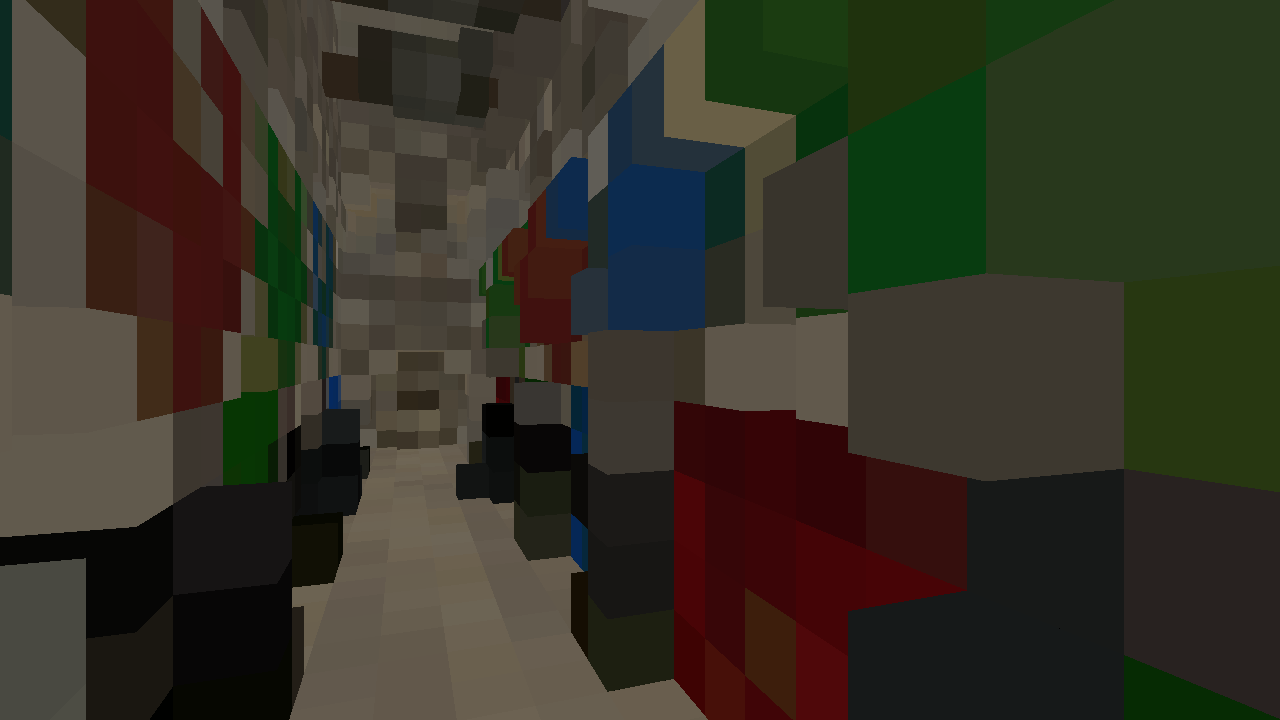
\includegraphics[width=\linewidth]{media/finals/albedo_v64.png}
	\end{subfigure}%
	\caption{Distintos niveles de detalle de una escena voxelizada.}
	\label{fig:voxelization_details}
\end{figure}

Este proceso de voxelización para las partes dinámicas de la escena debe ser realizado cada vez que sucede algún cambio sobre cualquier superficie que pertenece a un objeto dinámico en la escena. Por esta razón se requiere un algoritmo de voxelización de alto rendimiento para mantener tiempos interactivos.

\subsection{Voxelización Conservativa} % (fold)
\label{sub:voxelizacion_conservativa}
Nuestra implementación realiza voxelización conservativa de geometría de alto rendimiento totalmente por \ac{GPU} explotando características del pipeline de renderizado con OpenGL. Para esto se implementó el algoritmo de voxelización utilizando rasterizacion en hardware explicado en el libro OpenGL Insights por Cyril Crassin y Simon Green en \empty{Octree-Based Sparse
Voxelization Using the GPU
Hardware Rasterizer} \cite{CozziRiccio12}. 

Este algoritmo está basado en el trabajo de Zhang y otros en 2007 \cite{zhang2007conservative} para la voxelización conservativa utilizando la \ac{GPU} y el trabajo de Hasselgren y otros en 2005 \cite{hasselgren2005conservative} sobre rasterización conservativa.

Para maximizar el área de rasterización la idea es proyectar cada triangulo utilizando proyección ortogonal por cada eje direccional. El eje dominante es escogido según la normal del plano definido por los vértices del triángulo.

\begin{figure}[H]
	\centering
	\captionsetup{justification=centering}
	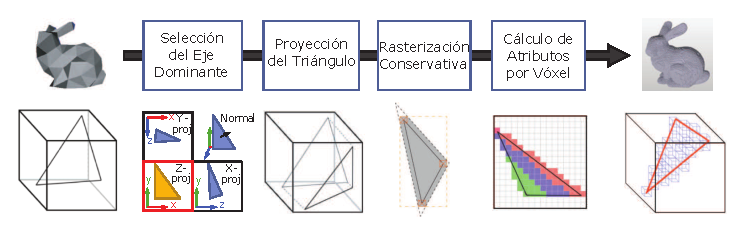
\includegraphics[width=\linewidth]{media/voxelization_pipeline.eps}
	\caption{Descripción del pipeline de voxelización.}
\end{figure}
 
Por cada triangulo proyectado es necesario generar un polígono delimitante un poco más grande que el triángulo para garantizar la voxelización conservativa. Este polígono debe permitir que por cualquier triangulo proyectado tocando un pixel este va obligatoriamente a tocar el centro de este pixel, por tanto el pipeline de rasterización generara fragmentos para este triángulo. El polígono se genera expandiendo cada vértice del triángulo hacia afuera utilizando el procesador de geometria o \emph{geometry shader}. El polígono delimitante no sobreestima la cobertura del triángulo por tanto este no tiene forma de triángulo. Los fragmentos excedentes de este polígono son descartados en el procesador de fragmentos o \emph{fragment shader} utilizando un cuboide delimitante.

\begin{figure}[H]
	\centering
	\captionsetup{justification=centering}
	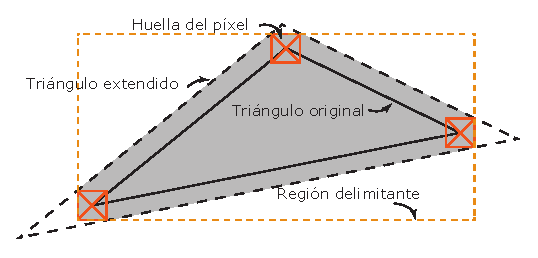
\includegraphics[width=0.7\linewidth]{media/conservative_triangle.eps}
	\caption{Polígono delimitante de un triángulo utilizado para rasterización conservativa.}
\end{figure}

% subsection voxelizacion_conservativa (end)
% section voxelizacion (end)

\subsection{Composicion de Fragmentos y Voxeles}

Una vez que los fragmentos han sido generados en el \emph{fragment shader}, los valores deseados puede ser almacenados en una textura 3D utilizando operaciones de escritura que provee la extensión \emph{{GL\_ARB\_shader\_image\_load\_store}} en OpenGL \cite{ImageLoadStore}. Sin embargo múltiples fragmentos de diferentes triángulos puede caer sobre una misma posición en esta textura 3D. Bajo el ambiente paralelo del \emph{fragment shader} no es posible saber el orden en que los fragmentos son creados y procesados, esto se traduce en resultados arbitrarios cada vez que se revoxeliza la escena.

Para solventar este problema se utilizaron operaciones atómicas proveídas por la misma extensión citada anteriormente. En nuestra implementación los valores necesarios a almacenar en vóxeles son normal, albedo y emisión. Una operación coherente y sencilla con respecto a estas propiedades en el espacio que envuelve un vóxel es un promedio.

\subsection{Voxelización Dinámica} % (fold)
\label{sub:voxelizacion_dinamica}
Para escenas complejas y densas en geometría poligonal el proceso de voxelización puede tomar considerable tiempo de ejecución afectando el rendimiento general del algoritmo si la escena necesita ser revoxelizada constantemente. Es por esto conveniente separar la voxelización de superficies estáticas y dinámicas en escena. La idea es voxelizar la parte estática de la escena una sola vez mientras que la parte dinámica es revoxelizada solo cuando sea necesario o constantemente por frame.

En nuestra implementación no se utiliza un octree disperso para almacenar los vóxeles sino texturas 3D. La separación entre valores estáticos y dinámicos bajo el esquema de un octree consiste en dividir el árbol en una parte dinámica y una parte estática. Considerando la cualidad dispersa de esta estructura esto no es de gran peso en memoria. 

Utilizando texturas 3D esto sería equivalente en nuestra implementación a generar en vez de tres texturas para almacenar albedo, normal y emisión se generarían seis. Tres de estas para la parte estática y tres para la parte dinámica. Esto es extremadamente ineficiente en memoria. Para evitar la creación de estas texturas se utiliza un volumen extra que permite indicar que vóxel forma parte de la parte estática y cuál no. Durante el proceso de voxelización dinámica solo los fragmentos que se encuentran dentro del espacio de un vóxel dinámico pueden escribir sobre la textura 3D.
% subsection voxelizacion_dinamica (end)
